In computational linear algebra, we would spend a lot of time in matrix equations or expressions like $Ax = b$. However, for large matrices  $A$, it is always difficult and inefficient to find the value of $x$, if we try finding the inverse of $A$ directly. So what we want to do is to "transform" our $A$ into smaller building blocks with specific properties, and use their properties of them to make the equation easier to solve. 

\medskip
\noindent The transformations, should preserve the correctness in matrix calculations (be sufficiently free from truncation errors, as said in the \href{https://comp-lin-alg.github.io/L2_QR_factorisation.html#what-is-the-qr-factorisation}{\textbf{Introduction}} of Chapter 2), and be efficient enough to perform. Here, let us talk about the very first transformation, the \textbf{QR Factorisation}. 
\medskip

\noindent You might have seen this in your year 2 \href{https://github.com/Imperial-MATH50003/MATH50003NumericalAnalysis}{Numerical Analysis} Course, and make some progress in implementation using Julia or Python. We would do some recap and dig further into algorithm stability, and/or time complexities with different ways of implementations.
\newpage
\section{QR Factorisation Concept}%
\begin{definition}[Complete QR Factorisation]
  The \textbf{Complete QR Factorisation} is defined as the processing of decomposing an arbitrary matrix $A \in \mathbb{C}^{m \times  n}$ to the form
  \[
    A = QR \text{ where } Q \text{ unitary } \in \mathbb{C}^{m \times m}, R  \text{ upper triangular } \in \mathbb{C}^{m \times n}
  .\]
\end{definition}
Without loss of generality we consider $m > n$, and have:
\[
\underset{\begin{array}{c}\\ A \end{array}}%
{
\begin{pmatrix}
  a_{11} & a_{12} & \ldots & a_{1n} \\
  a_{21} & a_{22} & \ldots & a_{2n} \\
  \vdots & \vdots & \ddots & \vdots \\
  a_{m1} & a_{m2} & \ldots & a_{mn}
\end{pmatrix}
}
=
\underset{\begin{array}{c}\\ Q \end{array}}%
{
\begin{pmatrix}
  q_{11} & \ldots & q_{1n} & \ldots & q_{1m} \\
  q_{21} & \ldots & q_{2n} & \ldots & q_{2m}\\
  \vdots & \ddots & \vdots & \ddots & \vdots\\
  q_{m1} & \ldots & q_{mn} & \ldots & q_{mm}
\end{pmatrix}
}
\begin{spmatrix}{R}
  r_{11} & r_{12} & \ldots & r_{1n} \\
  0 & r_{22} & \ldots & r_{2n} \\
  0 & 0 & \ldots & r_{3n} \\
  \vdots & \vdots & \ddots & \vdots \\
  0 & 0 & \ldots & r_{nn} \\
  \vdots & \vdots & \ddots & \vdots \\
  0 & 0 & \ldots & 0
\end{spmatrix}
\]
Note that, the term $q_{ik}r_{kj}$ would always give out 0 when $k > n$ and make no contribution to the value of  $a_{ij}$. Therefore, we could only consider the first $n$ columns of $Q$ and the first $n$ rows of $R$ as the result of factorisation.

\begin{definition}[Reduced QR Factorisation]
  The \textbf{Reduced QR Factorisation} is defined as the processing of decomposing an arbitrary matrix $A \in \mathbb{C}^{m \times  n}$ to the form
  \[
    A = \hat{Q}\hat{R} \text{ where } \hat{Q} \text{ unitary } \in \mathbb{C}^{m \times n}, \hat{R}  \text{ upper triangular } \in \mathbb{C}^{n \times n}
  .\]
  where \(\hat{Q}\), \(\hat{R}\) are sub-matrices of the  complete factorisation results \(Q\), \(R\).
\end{definition}
We are mainly talking about the \textbf{reduced} case of QR factorisation in this chapter, but do think about the complete case when doing exercises.

\subsection*{Exercise 2.3: Find an orthonormal basis of the orthogonal complement of a subspace}
\addcontentsline{toc}{subsection}{Exercise 2.3: Find an orthonormal basis of the orthogonal complement of a subspace}
\subsubsection*{Problem Description}%
\label{ssub:problem_description}

Given a set of vectors $ \{v_1, v_2, \ldots, v_n\}$ spans subspace $U \subset \mathbb{C}^{m}$, we need to find an orthonormal basis of its orthogonal complement $U^{\bot}$, defined as:
\[
U^{\bot} = \{x \in \mathbb{C}^{m}: \forall u \in U, x^{*}u = 0\} 
.\] 
Implement this as a function \href{https://comp-lin-alg.github.io/cla_utils.html#cla_utils.exercises2.orthog_space}{\texttt{exercises2.orthog\_space()}}. \medskip

\subsubsection*{Hints}
\begin{enumerate}
  \item Consider the condition \(\forall u \in U, x^{*}u = 0\), can we consider the elements in a smaller \textbf{subset of \(U\)} rather than all elements in \(U\) to simplify the satisfying criteria? If so, what is the subset?
  \item You might find the matrix \(Q\), \(R\) from complete factorisation useful for answering the question above.    
  \item Consider the matrix \(Q\) obtained from the \textbf{complete QR factorisation}, what is the relationship between any two columns of \(Q\)?  
  \item You might want to use the numpy-based QR factorisation routine \texttt{numpy.linalg.qr()}.
\end{enumerate}
If you have the answer to the questions above, you have already got the key to solving this problem. Pause here for a moment to think about how to obtain the orthonormal basis of \(U^{\bot}\). Feel free to read my explanation on the next page if you get confused. \medskip

\noindent \textbf{Remember to check your implementation passes the provided test cases.}
\newpage

\subsubsection*{Spoil Alert \ldots There is a way you could figure out the problem:}%
\begin{itemize}
\item The first thing we need to figure out is, we are finding the vectors that are \textbf{orthogonal to the basis} of \(U\). This could be obtained by the first \(n\) columns in matrix \(Q\) from the complete QR of \(U\).
\item Then we consider the matrix \(Q\). Given that $Q$ is unitary, we would see all column vectors are orthogonal to each other by expanding
  \[
    [Q^*Q]_{ij} = q_i^*q_j = \delta_{ij} = \left\{
      \begin{array}{l}
      0 \text{ when $i \neq j$} \\
      1 \text{ when $i = j$}
      \end{array}
    \right.
  .\] 
  \item We need to find the vectors that are orthogonal to the first \(n\)  column vectors in $Q$, i.e. columns of \(\hat{Q}\). And we could see the remaining $m - n$ columns in  $Q$ are indeed orthogonal to any vector in the first n columns, by the mutual orthogonality mentioned above. 
  \item Therefore, what we need to do is just to find the \textbf{last} $m - n$ \textbf{columns} from $Q$, which should should be the basis of the orthogonal complementary $U^{\bot}$. \checked
\end{itemize}

\newpage
\section{QR Factorisation by Classical Gram-Schmidt}%
We have already seen the concept of QR factorisation, and one of the applications through the previous exercise. Then we are going to explore what exactly happens in this factorisation, via algorithms. The first implementation we would discuss would be the \textbf{classical Gram-Schmidt algorithm}. The algorithm itself is straightforward:
\begin{algorithm}
  \caption{Classical Gram-Schmidt Algorithm}
  \begin{algorithmic}[1]
  \Procedure{GS\_classical}{A}
    \State initialise \(Q, R\)  as empty matrices
    \For{ \(j = 1\) to \(n\)}
      \State \(v_j = a_j\)
      \For{ \(i = 1\) to \(j - 1\)}
        \State \(r_{ij} = q_i^{*}a_j\)
        \State \(v_j = v_j - r_{ij}q_i\)
        \Comment{Remove components of existing \(q_i\) from \(v_j\)}
      \EndFor
      \State \(r_{jj} = \|v_j\|\)  
      \State \(q_j = \frac{v_j}{\|v_j\|}\)
      \Comment{Finish constructing a new basis vector \(q_j\)}
    \EndFor
    \State \Return \(Q, R\)
  \EndProcedure
  \end{algorithmic}
\end{algorithm}

\noindent However, the algorithm might look no sense at all since we haven't discussed the maths behind it so far. Here we look backwards to see how vectors $ \{a_i\} $ factorised to orthonormal vectors $ \{q_i\} $. \medskip

\noindent Just expand $A = QR$ by arithmetic:

 \[
   A = QR \implies \begin{pmatrix} a_1 & a_2 & \ldots & a_n \end{pmatrix} = 
   \begin{pmatrix} 
     q_1 & q_2 & \ldots & q_n 
  \end{pmatrix} 
   \begin{pmatrix} 
     r_{11} & r_{12} & \ldots & r_{1n} \\ 
     0 & r_{22} & \ldots & r_{2n} \\
     \vdots & \vdots & \ddots & \vdots \\
     0 & 0 & \ldots & r_{nn}
   \end{pmatrix}  
.\] 
So we could see the value of any column vector $a_j$ via column-space interpretation and get:
\[
  a_j = 
   \begin{pmatrix} 
     q_1 & q_2 & \ldots & q_j & \ldots & q_n 
  \end{pmatrix} 
  \begin{pmatrix} r_{1j}\\ r_{2j} \\ \vdots\\ r_{jj} \\ 0 \\ \vdots \\ 0 \end{pmatrix}
\] 
\[
  = r_{1j} q_1 + r_{2j}q_2 + r_{3j}q_3 + \ldots + r_{jj}q_j + 0 \cdot q_{j + 1} + \ldots + 0
  = \sum_{i=1}^{j} r_{ij}q_i
.\] 
Starting with $a_1$, we could see that:
 \[
a_1 = r_{11} q_1
.\] 
and in this expression we could observe $q_1$ is the unit vector parallel to $a_1$, so $r_{11}$ and $q_1$ should have the value
\[
r_{11} = \|a_1\| \text{ and } q_1 = \frac{a_1}{\|a_1\|} = \frac{a_1}{r_{11}}
.\]
Then consider $a_2$ from the summation expression above:
 \[
a_2 = r_{12}q_1 + r_{22}q_2
.\]
But we don't know how to get the value of $r_{12}$ yet. Since we know $a_2 = r_{22}q_2 + r_{12}q_1$, and here is the trick to find \(r_{12}\) by using \(q_1\)  :
\[
  q_1^* a_2 = r_{22}(q_1^{*}q_2) + r_{12}(q_1^{*}q_1) = r_{22} \cdot 0 + r_{12} \cdot 1 = r_{12}
.\]
and to get the value of $q_2$ and $r_{22}$, we remove the component of $q_1$ from $a_2$ and we could get:
\[
    v_2 = a_2 - r_{12}q_1 = r_{22}q_2 \implies 
    \left\{
      \begin{array}{l}
      r_{22} = \|v_2\| \\
      q_2 = \frac{v_2}{\|v_2\|} = \frac{v_2}{r_{22}}
      \end{array}
    \right.
.\]
Then we should have an orthonormal set $ \{q_1, q_2\} $, and we could compute corresponding $q_3$ and scale factor $r_{i3}$s in a similar approach. \medskip

\noindent As we repeat these steps iteratively, we could compute the value of $q_4, q_5, \ldots$ until $q_n$, and also the coefficients \(r_{ij}\). And more generally, given matrix \(A \in \mathbb{C}^{m \times n}\), we could compute the entries of \(Q \in \mathbb{C}^{m \times  n}, R \in \mathbb{C}^{n \times  n}\) with the following formula:
\[
  q_j = \frac{v_{j}}{\|v_{j}\|}
\]
\[
  r_{ij} = \left\{
    \begin{array}{ll}
    q_{i}^{*}a_{j} & i < j\\
    \|v_{j}\| & i = j\\
    0 & \text{otherwise}
    \end{array}
  \right.
  \]
  where
  \[
    v_{j} = \left\{
      \begin{array}{ll}
        a_{j} & i = 1\\
        a_{j} - \sum_{k=1}^{j - 1} r_{kj}q_{k} = a_{j} - \sum_{k=1}^{j - 1} (q_{k}q_{k}^{*})a_{j} & \text{otherwise}
      \end{array}
      \right.
      \]
      Now the algorithm above should be easy for you to understand. \checked

\noindent \textbf{Important! Please make sure you understand the gist behind the contents below.}  The expressions of \(r_{ij}\) and \(v_j\) look messy and complex to implement in python. Here we have a concise and elegant way to find the values of \(r_{ij}\) and \(v_j\) via matrix products.
\[
  r_j = \begin{pmatrix} r_j^{(j - 1)} \\ r_{jj} \\ 0 \\ \vdots \\ 0\end{pmatrix} = \begin{pmatrix} Q_{(j - 1)}^{*}a_j \\ \|v_j\| \\ 0 \\ \vdots \\ 0\end{pmatrix}
  \]
  where \(Q_{j - 1} = \begin{pmatrix} 
  q_1 & \dots & q_{j - 1} 
\end{pmatrix} \) and \(r_j^{(j - 1)} = \begin{pmatrix} 
  r_{1j} & \dots & r_{(j-1)j}
\end{pmatrix} \), with   
\[
  v_j = a_j - Q_{j - 1}r_j^{(j - 1)} = a_j - Q_{j - 1}(Q_{j - 1}^{*}a_j) = (I - Q_{j - 1}Q_{j - 1}^{*})a_j
\]
Note that the \(^{*}\) here \textbf{refers to the adjoint of a matrix}, not the scalar multiplication!
\textbf{Do pause here for a while to make sure you could show the expressions above by yourself.} \medskip

\noindent 
You can see we are now eliminating the index \(i\) in every expression by replacing the summation with matrix products. This is essential since you can get rid of one for-loop with variable \(i\)  in the algorithm above, and use NumPy-based matrix multiplication. \smallskip

\noindent Since we've seen the fact that using matmul in NumPy is more efficient than using for loops, you should pay more attention to using more "vectorized operations" like matmul, and \textbf{reduce for loops as much as possible. }

\noindent Here is the optimised version of the classical Gram-Schmidt algorithm, \textbf{which is not mentioned by the lecturer} but you would \textbf{lose marks if not optimised.}
\begin{algorithm}
  \caption{Classical Gram-Schmidt Algorithm, optimised}
  \begin{algorithmic}[1]
  \Procedure{GS\_classical\_optimised}{A}
    \State initialise \(Q, R\)  as empty matrices
    \For{ \(j = 1\) to \(n\)}
      \State \(r_j^{(j - 1)} = Q_{(j - 1)}^{*}a_j\)
      \State \(v_j = a_j - Q_{j - 1}r_j^{(j - 1)}\)
      \State \(r_{jj} = \|v_j\|\)
      \State \(q_j = \frac{v_j}{\|r_{jj}\|}\)    
    \EndFor
    \State \Return \(Q, R\) 
  \EndProcedure
  \end{algorithmic}
\end{algorithm}

\newpage
\noindent To let you have a more direct sense of classical Gram-Schmidt, \autoref{cgs} would demonstrate the flow of the classical Gram-Schmidt Algorithm. 
\begin{figure}[htp]
  \centering
  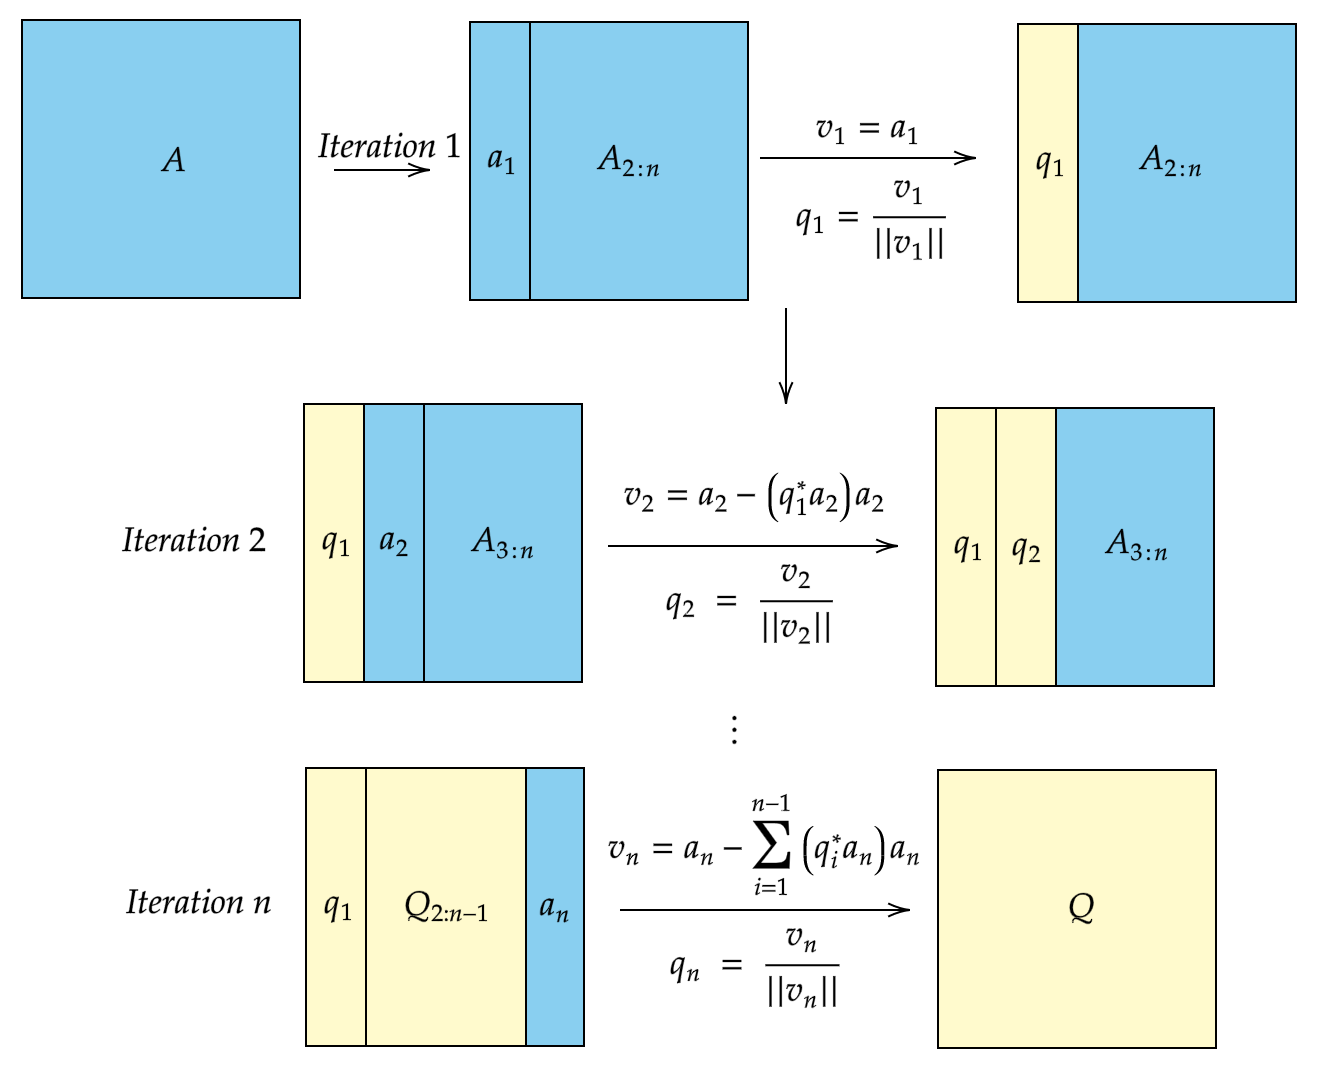
\includegraphics[width=\textwidth]{imgs/cgs.png}
  \caption{Classical Gram-Schmidt Algorithm Demonstration}
  \label{cgs}
\end{figure}

\noindent The only difference between the algorithm and \autoref{cgs} is I didn't create another array to store column-vectors of \(Q\) but in the sense of "converting" \(A\)  to \(Q\)  column-wise.
\newpage
\subsection*{Exercise 2.4: Implement the Classical Gram-Schmidt Algorithm}
\addcontentsline{toc}{subsection}{Exercise 2.4: Implement the Classical Gram-Schmidt Algorithm}
\subsubsection*{Problem Description}%
Here you need to implement the classical Gram-Schmidt algorithm from the derivation above in your function \href{https://comp-lin-alg.github.io/cla_utils.html#cla_utils.exercises2.GS_classical}{\texttt{exercises2.GS\_classical()}}. Note that instead returning matrices \(Q\) and \(R\) from the function, you need to change original matrix \(A\) to \(Q\) 'in-place' (which is in the way I demonstrated in \autoref{cgs}) and return \(R\) only.
\subsubsection*{What to do}
There is not too much to talk about in this exercise. However, two things are still worth mentioning:
\begin{enumerate}
  \item You are asked to change \(A\)  to \(Q\)  "in-place", which is not mentioned in the pseudo-code above. A good initiative to achieve this is to initialise \texttt{Q = A} in your function and follow the optimised algorithm to write your code. 
  \item When creating empty or zero matrices with NumPy, the matrices would not be initialised as complex matrices. You might find specifying \texttt{dtype=np.complex128} or \texttt{dtype=A.dtype} useful in your code implementation.  
\end{enumerate}
The main task for you now is to not be confused between indexes in maths formulas and Python (starting from 0). Try using 'vectorized' operations in your implementation, e.g. matrix multiplication rather than additional loops. \medskip

\noindent \textbf{Remember to check your implementation passes the provided test cases.}

\section{QR Factorisation by Modified Gram-Schmidt}
This part is the modification of classical Gram-Schmidt and contains two coding exercises. The initiative we want to make a modified version of classical Gram-Schmidt is due to the instability of classical GS. Here is the demonstration:\medskip

\noindent Let us say we have obtained \(Q, R\) from classical Gram-Schmidt, and mathematically we should have \(QR = A\). But since there are lots of rounding errors from the inexact arithmetic when this algorithm runs on computers, the entries of \(Q, R\)  are "polluted" so it is not necessarily correct for the equation \(QR = A\) when we do factorisation with classical GS. \medskip

\noindent Therefore the mathematicians propose a quick fix to the classical GS algorithm, and we called the modified version as \textbf{modified Gram-Schmidt}. The algorithm goes in this way:

\begin{algorithm}
\caption{Modified Gram-Schmidt Algorithm}
\label{mgs-algorithm}
\begin{algorithmic}[1]
\Procedure{GS\_modified}{A}
  \State initialise \(Q, R\)  as empty matrices
  \For{ \(i = 1\) to \(n\)}
    \State \(v_i = a_i\)
    \State \(r_{ii} = \frac{v_i}{\|v_i\|}\)  
    \For{ \(j = i + 1\) to \(n\)}
      \State \(r_{ij} = q_i^{*}v_j\)
      \State \(v_j = v_j - r_{ij}q_i\)
      \Comment{Remove components of \(q_i\) from all \(v_j\)s}
    \EndFor
    \Comment{Finish constructing a new basis vector \(q_j\)}
  \EndFor
  \State \Return \(Q, R\)
\EndProcedure
\end{algorithmic}
\end{algorithm}

\noindent To let you have a more direct sense of modified Gram-Schmidt, \autoref{mgs} would demonstrate the flow of the modified Gram-Schmidt Algorithm. \medskip
\begin{figure}[H]
  \centering
  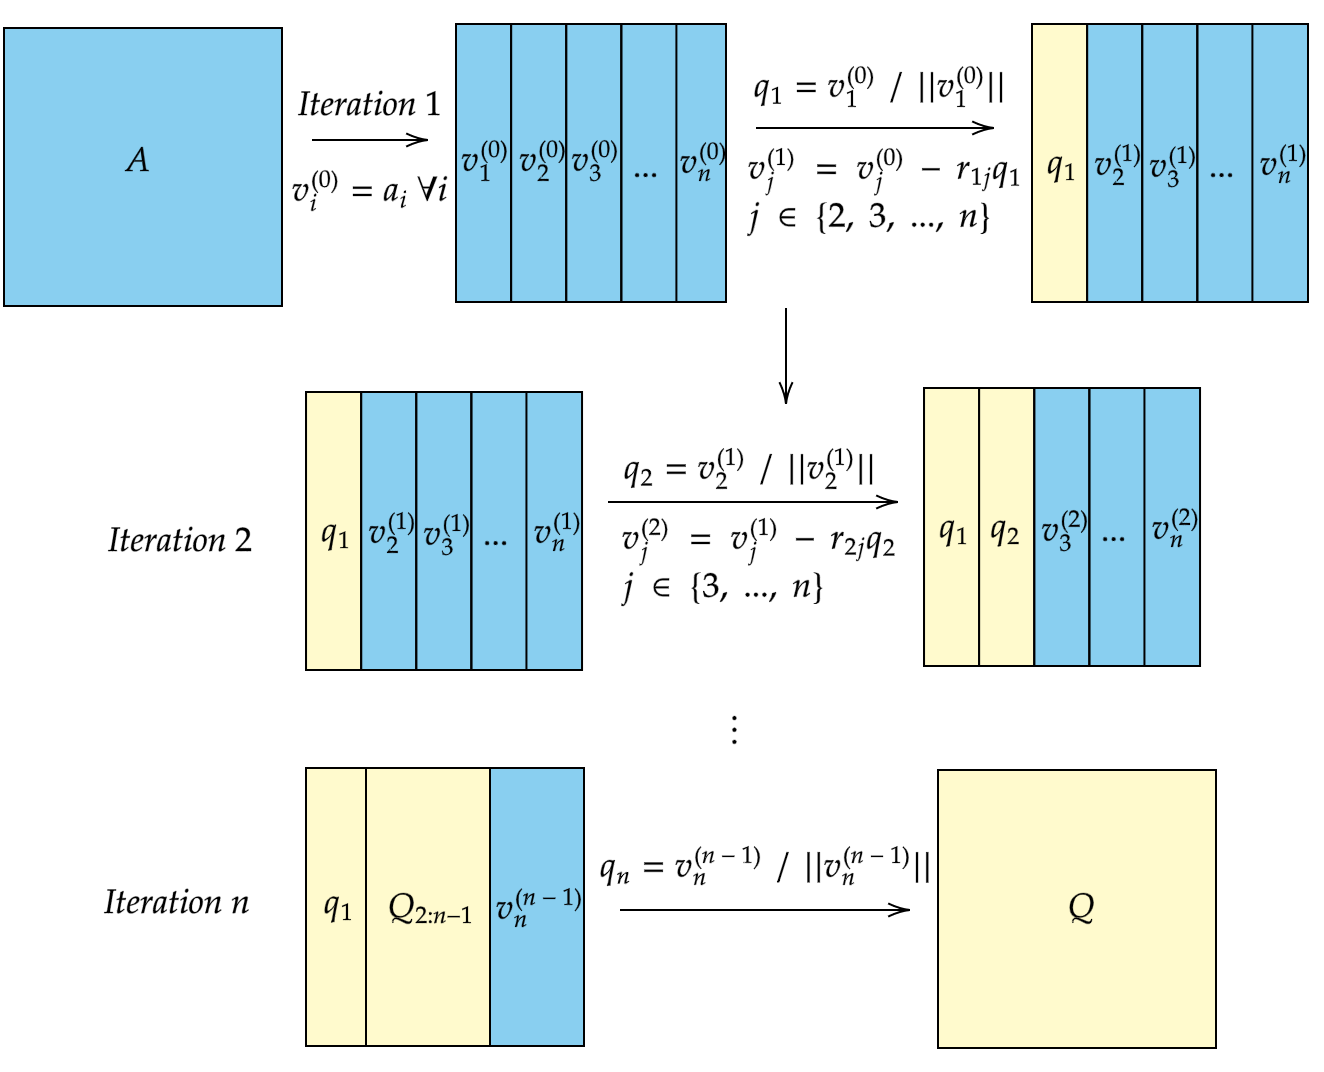
\includegraphics[width=0.9\textwidth]{imgs/mgs.png}
  \caption{Modified Gram-Schmidt Algorithm Demonstration}
  \label{mgs}
\end{figure}
\noindent You might find it confusing that, there are also superscripts in \(v_k\)  in \autoref{mgs} above, e.g. \(v_3^{(2)}\). The notation \(v_k^{(i)}\)  here is just for demonstrating the updated value of column vector \(v_k\) after iteration \(i\). 

\noindent For simplicity, I will ignore the superscripts \(^{(i)}\) in \(v_k\) in the following explanations, and I hope you could still understand the upcoming contents. \medskip

\noindent Essentially the modified GS and the classical GS have the same effect in factorisation. Recall that in classical GS what we did in each iteration \(k\) is, \textbf{set the vector \(v_k = a_k\), remove the components of found \(\{q_1, q_2, ..., q_{k - 1}\}\) from \(v_k\), set the normalised (and updated) \(v_k\) as \(q_k\), and add the obtained \(q_k\)  to the existing orthonormal set \(\{q_i\}\)} for the next iteration. However, what we did in the modified GS is, for each iteration \(k\), \textbf{I picked up the column vector \(v_k\), normalise it to obtain a basis vector \(q_k\), and remove the components of \(q_k\) from the vectors \(\{v_{k + 1}, ..., v_{n}\}\)} behind. \medskip

\noindent The two algorithms indeed have the same effect on an arbitrary matrix \(A\), and also have the same number of computational operations. However, the main difference is that in modified GS we define \(r_{ij} = q_i^{*}v_j\) rather than \(r_{ij} = q_i^{*}a_j\). In this case, \textbf{the rounding error} in finding \(r_{ij}\) would be \textbf{smaller} and the \textbf{algorithm will be more stable.} Click \href{https://math.stackexchange.com/questions/3913710/intuitive-explanation-of-why-the-modified-gram-schmidt-is-more-stable-than-the-c}{here} to see the explanation.\medskip

\noindent You might think now you should be ready for implementing this algorithm by yourself. However, from one of the gist in this course, \textbf{you should use avoid "additional" for loops as much as possible}. That is to say, you should consider if you could reduce the number of "for loops" in the algorithm shown in the class/on the website. Pause here for a while to think about it, and go to the next page for checking my solution to reduce no. of for-loops by introducing vectorized operations. 

\newpage
\noindent Consider the inner for-loop starting from \textbf{line 6 to line 9} in \autoref{mgs-algorithm}. Firstly we should see in this loop we computed the values \(\{r_{i(i + 1)}, r_{i(i + 2)}, ..., r_n\}\), by arithmetic we should see
\[
  r_i^{(i + 1, n)} = \begin{pmatrix} 
    r_{i(i + 1)} \\ r_{i(i + 2)} \\ \vdots \\ r_n
  \end{pmatrix}
  = 
  \begin{pmatrix} 
      q_i^{*}v_{i + 1} \\
      q_i^{*}v_{i + 2} \\
      \vdots \\
      q_i^{*}v_{n}
  \end{pmatrix}
  = \begin{pmatrix} 
     v_{i + 1}^{*}q_i & v_{i + 2}^{*}q_i & ... & v_{n}^{*}q_i
  \end{pmatrix}^{*}
\]
\[
  =
  (\begin{pmatrix} 
    v_{i + 1}^{*}q_i \\
    v_{i + 2}^{*}q_i \\
    \vdots \\
    v_{n}^{*}q_i
\end{pmatrix}^{\top})^{*}
  = ((V_{i + 1}^{*}q_i)^{\top})^{*} = ((V_{i + 1}^{*}q_i)^{*})^{\top} 
\]
\[
  = (q_i^{*}V_{i + 1})^{\top} = V_{i + 1}^{\top}\overline{q_i}
\]
where \(V_{i + 1} = \begin{pmatrix} 
    v_{i + 1} & v_{i + 2} & ... & v_{n}
\end{pmatrix} \)  and \(\overline{q_i}\) is the complex conjugate of \(q_i\). \medskip

\noindent Also we could see the component of \(q_i\)  is removed from \(\{v_{i + 1}, v_{i + 2}, ..., v_{n}\} \) in iteration \(i\). Recall the definition of outer product \(uv^{\top}\) and we should see
\[
  V_{i + 1} = V_{i + 1}
  - \begin{pmatrix} 
    r_{i(i + 1)}q_i & r_{i(i + 2)}q_i & ... & r_{in}q_i 
  \end{pmatrix} 
\]
\[
  = V_{i + 1} - q_i \begin{pmatrix} 
    r_{i(i + 1)} \\
    r_{i(i + 2)} \\
    \vdots \\
    r_{in}
  \end{pmatrix}^{\top}
  = V_{i + 1} - q_i (r_i^{(i + 1, n)})^{\top}
\]
Therefore, you now have the optimised version of the modified Gram-Schmidt algorithm, which is not mentioned by the lecturer but you would lose marks if not optimised.

\begin{algorithm}
  \caption{Modified Gram-Schmidt Algorithm, optimised}
  \label{mgs-algorithm-optimised}
  \begin{algorithmic}[1]
  \Procedure{GS\_modified\_optimised}{A}
    \State initialise \(Q, R\)  as empty matrices
    \For{ \(i = 1\) to \(n\)}
      \State \(v_i = a_i\)
      \State \(r_{ii} = \frac{v_i}{\|v_i\|}\)
      \State \(r_i^{(i + 1, n)} = V_{i + 1}^{\top}\overline{q_i}\)
      \State \(V_{i + 1} = V_{i + 1} - \overline{q_i} (r_i^{(i + 1, n)})^{\top}\)    
    \EndFor
    \State \Return \(Q, R\)
  \EndProcedure
  \end{algorithmic}
  \end{algorithm}

\subsection*{Exercise 2.5: Implement the Modified Gram-Schmidt Algorithm}
\addcontentsline{toc}{subsection}{Exercise 2.5: Implement the Modified Gram-Schmidt Algorithm}
\subsubsection*{Problem Description}%
You are now asked to implement the modified Gram-Schmidt algorithm in \href{https://comp-lin-alg.github.io/cla_utils.html#cla_utils.exercises2.GS_modified}{\texttt{exercises2.GS\_modified()}}. You should be able to implement it with the minimum amount of loops from reading the optimised algorithm above. \medskip

\noindent \textbf{Remember to check your implementation passes the provided test cases.}

\section{Modified Gram-Schmidt Algorithm with Triangular Orthogonalisation}
From \autoref{mgs} you should see how modified Gram-Schmidt works iteratively. However, from another perspective, we could consider each iteration \(k\) as a transformation represented by matrix \(R_k\). Let us say $\hat{A}_0 = A$ and $\hat{A}_{k} = \hat{A}_{k - 1}R_k$, the transformation \(R_k\) should satisfy the following criteria:
\[
  \hat{A}_0 = \begin{pmatrix} v_{1}^{(0)} & v_{2}^{(0)} & \ldots & v_{n}^{(0)}\end{pmatrix} = A
\] and 
\[
  \hat{A}_{k} = \begin{pmatrix} v_1^{(k)} & v_2^{(k)} & \ldots & v_{n}^{(k)} \end{pmatrix} = \hat{A}_{k - 1}R_{k}
\] 
\begin{enumerate}
  \item The first $k - 1$ columns in $\hat{A}_{k - 1}$ and $\hat{A}_{k}$ should be the same after transformation. i.e. 
  \[
    \begin{pmatrix} v_1^{(k - 1)} & \ldots & v_{k - 1}^{(k - 1)} \end{pmatrix} = \begin{pmatrix} v_1^{(k)} & \ldots & v_{k - 1}^{(k)} \end{pmatrix} 
  \] 
  \item The $k$-th column in $\hat{A}_{k}$ is the normalised vector of column $k$ in $\hat{A}_{k - 1}$. i.e.
    \[
    v_{k}^{(k)} = \frac{v_{k}^{(k - 1)}}{\|v_{k}^{(k - 1)}\|}
    \] 
  \item The last $(n - k)$ columns in $\hat{A}_{k}$ is transformed from $\hat{A}_{k - 1}$ where
    \[
      v_{i}^{(k)} = v_{i}^{(k - 1)} - r_{ki} \frac{v_k^{(k - 1)}}{\|v_{k}^{(k - 1)}\|} = v_{i}^{(k - 1)} - \frac{r_{ki}}{r_{kk}}v_{k}^{(k - 1)} ~\forall i \in \{k + 1, k + 2, \ldots, n\} 
    \] 
    where
    \[
      r_{kk} = \|v_{k}^{(k - 1)}\|, r_{ki} = q_k^{*}v_{i}^{(k - 1)} = \frac{(v_k^{(k - 1)})^{*}v_{i}^{(k - 1)}}{\|v_{k}^{(k - 1)}\|}
    \]  
\end{enumerate}
Recall here we use the notation \(v_l^{(r)}\) for demonstrating the updated value of column vector \(v_l\) after iteration \(r\).
\begin{itemize}
  \item From the \textbf{Criteria 1} we could see that, when $1 \le  l \le  k - 1$, the $l$-th column vector of $\hat{R}_{k}$ should be the base vector $e_{l}$. i.e. the $r$-th element in vector $e_l$ is represented as the Kronecker delta $\delta_{lr}$.
  \item From the \textbf{Criteria 2} we could see that the $k$-th column vector of $ \hat{R}_{k}$ should be $\frac{e_k}{r_{kk}}$ in which $e_k$ follows the same definition as above.
  \item From the  \textbf{Criteria 3} we could see that the last $(n - k)$ columns of $\hat{R}_{k}$ (say the column $i$ is called $r_{k}^{(i)}$) should be in the form
    \[
      [r_{k}^{(i)}]_j = \left\{
        \begin{array}{ccl}
          1 &~ & $j = i$ \\
          -\frac{r_{ki}}{r_{kk}} & ~&$j = k$ \\
          0 & ~&\text{otherwise}
        \end{array}
      \right.
    .\] 
\end{itemize}
Therefore, the matrix $\hat{R}_{k}$ should take the form when $k = 2$:
\[
  \hat{R}_{k} = \begin{pmatrix}
  1 & 0 & 0 & \ldots & 0 \\
  0 & \frac{1}{r_{22}} & -\frac{r_{23}}{r_{22}} & \ldots & -\frac{r_{2n}}{r_{22}} \\
  0 & 0 & 1 & \ldots & 0 \\
  \vdots & \ddots & \ddots & \ddots & \vdots \\
  0 & \ldots & 0 & \ldots & 1
\end{pmatrix} 
\]
i.e. A $n \times n$ identity matrix except row $k$ is filled starting from the diagonal element $r_{kk}$, where the diagonal element is $\frac{1}{r_{kk}}$ and the elements behind the element takes the form $-\frac{r_{ki}}{r_{kk}}$, where $i$ is the column index. In which case
\[
  \{-\frac{r_{ki}}{r_{kk}}\} = \begin{pmatrix} 
    - \frac{r_{k(k + 1)}}{r_{kk}} \\ -\frac{r_{k(k + 1)}}{r_{kk}} \\ \vdots \\ -\frac{r_{kn}}{r_{kk}}
  \end{pmatrix} = -\frac{1}{\|v_{k}^{(k - 1)}\|}\begin{pmatrix} 
    (v_k^{(k - 1)})^{*}v_{k + 1}^{(k - 1)} \\
    (v_k^{(k - 1)})^{*}v_{k + 2}^{(k - 1)} \\
    \vdots \\
    (v_k^{(k - 1)})^{*}v_{n}^{(k - 1)}
  \end{pmatrix} = -\frac{(V_{k + 1}^{(k - 1)})^{\top}\overline{v_k^{(k - 1)}}}{\|v_{k}^{(k - 1)}\|}
\]
where \(V_{k + 1}^{(k - 1)} = \begin{pmatrix} 
  v_{k + 1}^{(k - 1)} & v_{k + 2}^{(k - 1)} & ... & v_{n}^{(k - 1)}
\end{pmatrix} \). i.e. the last \(n - k\) cols of \(\hat{A}_{k - 1}\).  \medskip

\noindent You should also see that inductively the $\hat{Q}$ obtained from this method takes this form:
\[
\hat{Q} = A \hat{R}_1 \hat{R}_2 \ldots \hat{R}_n
\] 
And since every $\hat{R}_k$ is essentially an upper triangular matrix, so do their products. We know that the inverse of an upper triangular matrix is still upper triangular, so we could obtain $\hat{R}$ from the inverse of product $\prod_{k=1}^{n}\hat{R}_k$. \medskip

\noindent Also here we are using a series of \textbf{upper triangular} matrices to obtain an orthogonal matrix $\hat{Q}$, and this is the reason we called it \textbf{triangular orthogonalisation}. The algorithm with triangular orthogonalisation in modified Gram-Schmidt is shown below:

\begin{algorithm}[H]
  \caption{Get \(R_k\) for triangular orthogonalisation in modified GS}
  \label{mgs-get-r}
  \begin{algorithmic}[1]
  \Procedure{GS\_modified\_get\_R}{$\hat{A}_{k - 1}$, $k$} 
    \State initialise \(\hat{R}_k\)  as an identity matrix
    \State \(\hat{R}_{k}\)\texttt{[k, k]} \(= \|\hat{A}_{k - 1}\texttt{[:, k]}\|\)
    \State \(\hat{R}_{k}\)\texttt{[k, k + 1:]} \(=- \frac{\hat{A}_{k - 1}\texttt{[:, k + 1:]}^{\top} \overline{\hat{A}_{k - 1}\texttt{[:, k]}}}{\hat{R}_{k}\texttt{[k, k]}}\)       
    \State \Return \(\hat{R}_k\)
  \EndProcedure
  \end{algorithmic}
  \end{algorithm}
\noindent Note that some implementations of this algorithm will not explicitly mention \(\hat{A}_{k - 1}\) as the input parameter, instead the input parameter would be a general matrix \(A\). Keep this in mind and you might need this in exercise. 
\begin{algorithm}[H]
  \caption{Modified Gram-Schmidt with Triangular Orthogonalisation}
  \label{mgs-r}
  \begin{algorithmic}[1]
  \Procedure{GS\_modified\_R}{$A$} 
    \State \texttt{m, n = A.shape}
    \State initialise \(Q, R\) as \(A\) and an identity matrix
    \For{ \(k = 1\) to \(n\)}
      \State \(\hat{R}_k = \)  GS\_MODIFIED\_GET\_R\((A, k)\)
      \State \(Q = Q \hat{R}_{k}\)
      \State \(R = R \hat{R}_{k}\)     
    \EndFor
    \State \Return \(Q, R\)
  \EndProcedure
  \end{algorithmic}
  \end{algorithm}

  \subsection*{Exercise 2.7: Implement the \texttt{get\_R()} Function Modified GS}
  \addcontentsline{toc}{subsection}{Exercise 2.7: Implement the \texttt{get\_R()} Function Modified GS}
  \subsubsection*{Problem Description}%
  You are now asked to implement the modified Gram-Schmidt algorithm in \href{https://comp-lin-alg.github.io/cla_utils.html#cla_utils.exercises2.GS_modified_get_R}{\texttt{exercises2.GS\_modified\_get\_R()}}. You should be able to implement it with reference of \autoref{mgs-get-r}. \medskip
  
\noindent \textbf{Remember to check your implementation passes the provided test cases.}


 \bigskip

 \begin{center}
   \textit{\large End of Week 2}
 \end{center}
\newpage
\section{QR Factorisation with Householder Triangulation}
\subsection*{Before we start}
\textbf{This part is hard to understand} - I am saying this is because the materials were taught disappointedly when I learned this part. I found it harsh to understand it in one or two days, with the not well-organised materials on the course web page. \medskip

\noindent So I put lots of effort into re-organising the materials and trying to arrange the materials as a learning journey for you to easily understand this part. I am confident my version would be relatively easier to follow, with additional diagrams and explanations. Don't panic if you find this part difficult, I will always be there and we will finally figure out where the problems are.

\subsection*{Contents}
We have just seen how to use multiple upper triangular matrices $\hat{R}_{k}$ to convert a matrix $A$ to an orthogonal matrix $\hat{Q}$. Similarly, you might be thinking if we could use multiple unitary matrices $\hat{Q}_{k}$ to convert a matrix $A$ to an upper triangular matrix $R$. The answer is yes and the approach behind this idea is \textbf{Householder Triangulation}. \medskip

\noindent Suppose we have a series of \textbf{orthogonal matrices} $\hat{Q}_{k} \in \mathbb{C}^{m \times m}$, what we want to do to convert the matrix $A \in \mathbb{C}^{m \times n}$ to upper triangular $R \in \mathbb{C}^{m \times n}$ is simply
\[
\hat{Q}_{m}\hat{Q}_{m - 1}\ldots \hat{Q}_{2}\hat{Q}_1 A= R
\] 
and since the product of unitary matrices $\hat{Q}_{k}$ is also unitary, we could set $Q^{*} = \hat{Q}_{m}\hat{Q}_{m - 1}\ldots \hat{Q}_{2}\hat{Q}_{1}$. The answer to $Q \in \mathbb{C}^{m \times m}$ should be straightforward to get. You might also notice that using this approach could help us do \textbf{full QR Factorisation}. This property would let us see lots of applications of QR factorisation using householder triangulation. You can take the diagram below as a reference to the initiative.
\begin{figure}[H]
  \centering
  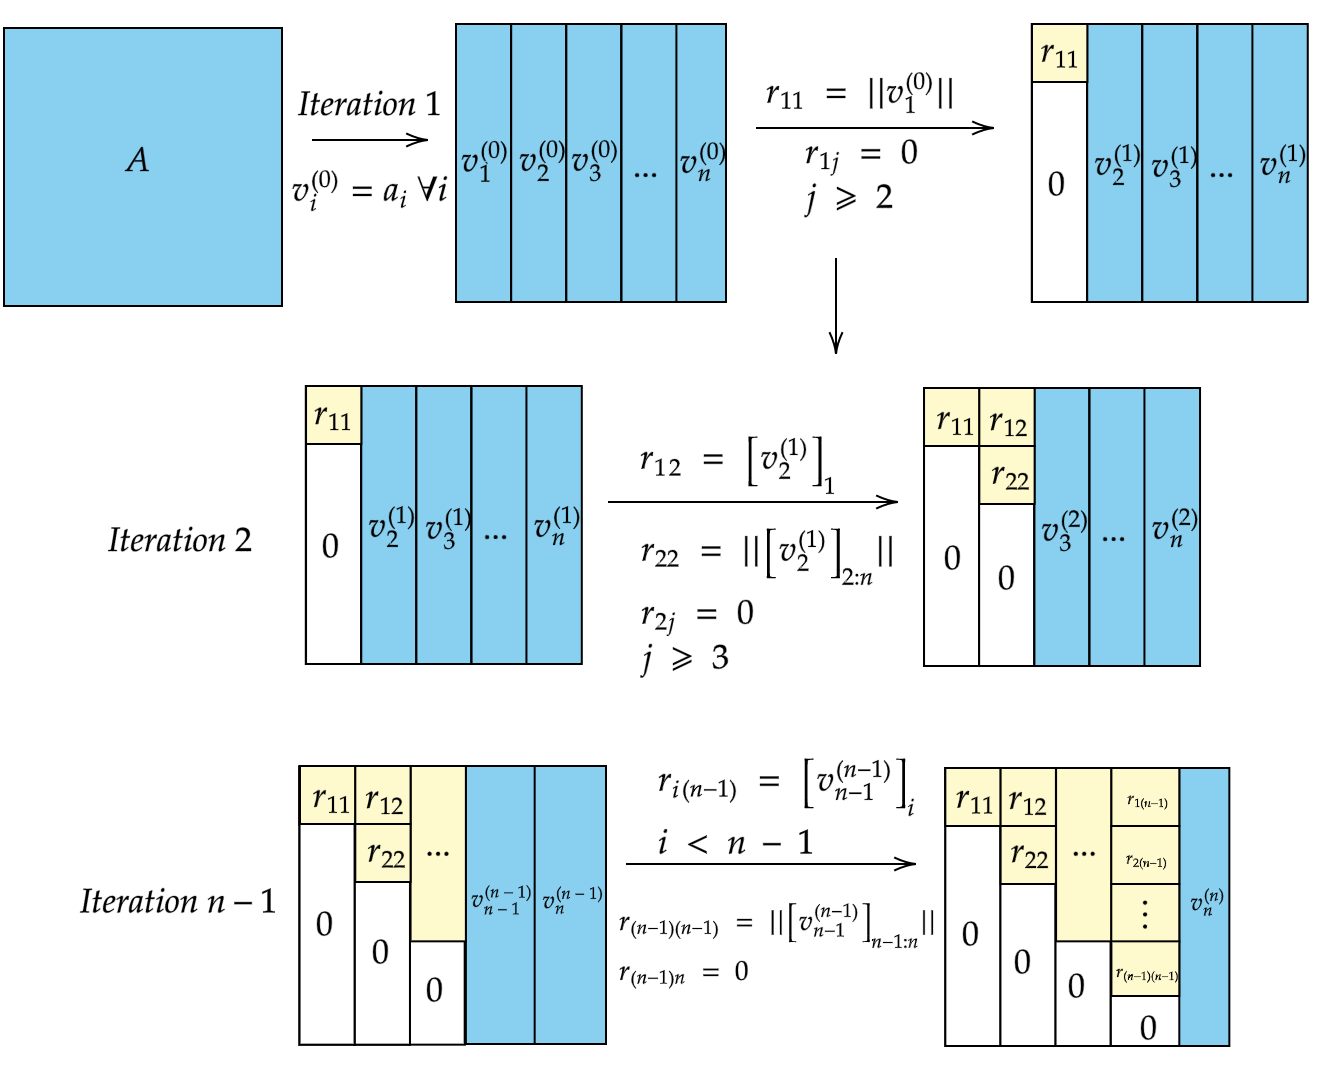
\includegraphics[width=0.7\textwidth]{./imgs/householder.png}
  \caption{An initiative to the Householder Triangulation}
  \label{fig:householder}
\end{figure}

\noindent However, how to define \(\hat{Q}_{k}\) is indeed the challenge we are facing. Let's suppose that \(\hat{A}_{k} = \hat{Q}_{k}\hat{A}_{k -1}\). The transformation \(\hat{Q}_{k}\) should satisfy the following basic conditions:

\begin{enumerate}
  \item To make the final matrix \(R\)  upper triangular, here we want \(\hat{Q}_k\) making the elements below \(k\)-th element in the \(k\)-th column of \(\hat{A}_k\) be 0. 
  \item Clearly, we don't want \(\hat{Q}_k\) to "pollute" the upper-triangular structure when multiplying with \(\hat{A}_{k -1 }\) to get \(\hat{A}_{k}\). Therefore, we need the first \((k - 1)\) columns in \(\hat{A}_{k}\) and \(\hat{A}_{k - 1}\) be the same.          
\end{enumerate}
These two conditions both points to one simple structure of \(\hat{Q}_k\), where
\[
  \hat{Q}_{k} = \begin{pmatrix} 
    I_{k - 1} & 0 \\
    0 & F_{k} 
  \end{pmatrix} 
\]
The matrix \(I\) refers to the identity matrix but \(F_{k}\) is still unknown. However when you choose an arbitrary vector \(a =  \begin{pmatrix} 
  a_1 & a_2 & ...a_{k - 1} & a_{k} & a_{m - 1} & a_{m} 
\end{pmatrix}^{\top} \) and try calculating the value of \(\hat{Q}_{k}a\), you should get
\[
  \hat{Q}_{k}a = \begin{pmatrix} 
    a_1 \\
    a_2 \\
    \vdots \\
    a_{k - 1} \\
    F_k a_{k:m}
  \end{pmatrix} 
\]
and the value of \(F_{k}a_{k:m}\) should be in the form \(\begin{pmatrix} 
  b & 0 & ... & 0 
\end{pmatrix}^{\top} \).

\noindent Here we will use a trick to set \(x = a_{k:m}\) and \(b = \|x\|\), you should see 
\[
  \|F_{k}x\| = \sqrt{(\|x\|^2 + 0^2 + ... + 0^2)} = \|x\|
\] and consequently \(F_kx = \pm \|x\|e_1\). \medskip

\noindent The \(+\) and \(-\) signs here are merely choices for constructing your \(\hat{Q}_{k}\), but the choice will affect the stability and accuracy of the algorithm, we will talk about the choice of signs later. Without the loss of generality, here we take the plus sign first. Now we need to find the exact structure of $F_{k}$, and here is a diagram for the intuition. 
\begin{figure}[H]
  \centering
  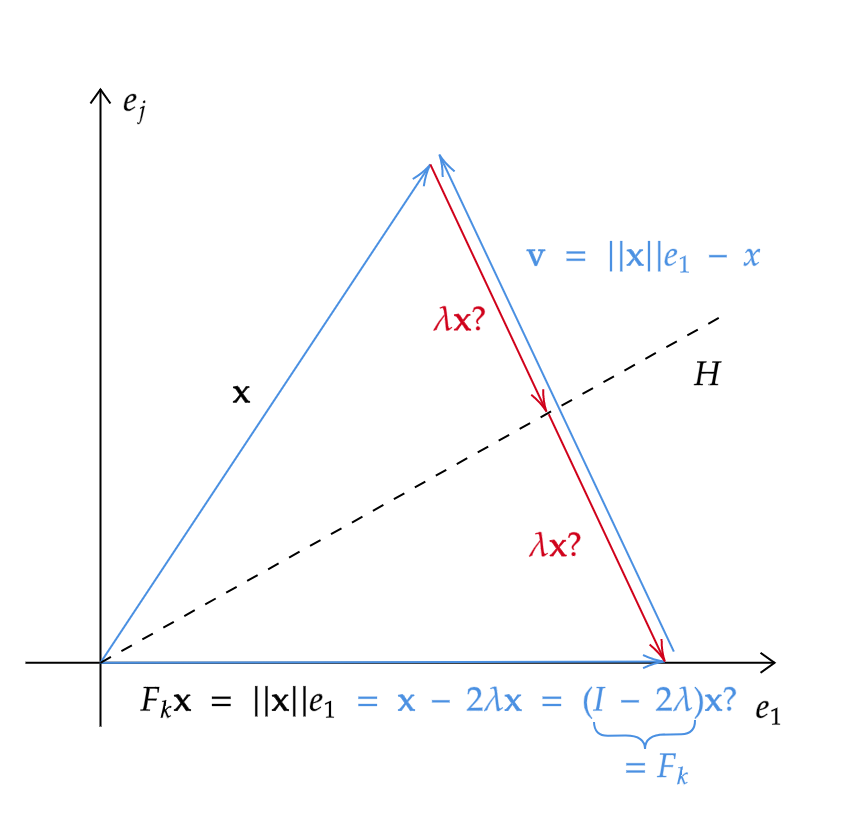
\includegraphics[width=0.7\textwidth]{./imgs/householder-reflector-initial.png}
  \caption{Finding Householder Reflector $F_k$}
  \label{fig:householder-reflector-initial}
\end{figure}
\noindent Essentially here I am trying to find a reflection between the original vector $x$ and $ \|x\|e_1$ about a hyper-plane $H$. The hyper-plane should bisect the vector between $x$ and $ \|x\|e_1$ into two equal parts. \medskip

\noindent Let us say the two equal vectors could be written in the form $\lambda x$ as shown in the diagram, then we should get the expression of  $F_kx = x - 2\lambda x = (I - 2\lambda)x$ and we could easily get the expression of $F_k = I - 2\lambda$. \medskip

\noindent Here we introduce a vector $v = \|x\|e_1 - x$. From the diagram above we could see the vector $\lambda x$ is the projection of  $x$ along $-v$ \textbf{with an opposite direction}. So we could see that
 \[
-\lambda x = \frac{(-v)^{*}x}{\|-v\|} \frac{-v}{\|-v\|} = \frac{v(v^{*}x)}{\|v\|^2} = \frac{vv^{*}}{v^{*}v}x
\]
Therefore we could get $-\lambda = \frac{vv^{*}}{v^{*}v}$, and the vector $F_kx$ is in the form
\[
F_kx = (I - 2\lambda)x = (I - 2\frac{vv^{*}}{v^{*}v}) x \implies F_k = I - 2\frac{vv^{*}}{v^{*}v}
\] 
and the detailed graphical explanation goes as follows in \autoref{fig:householder-reflector-complete}:
\begin{figure}[H]
  \centering
  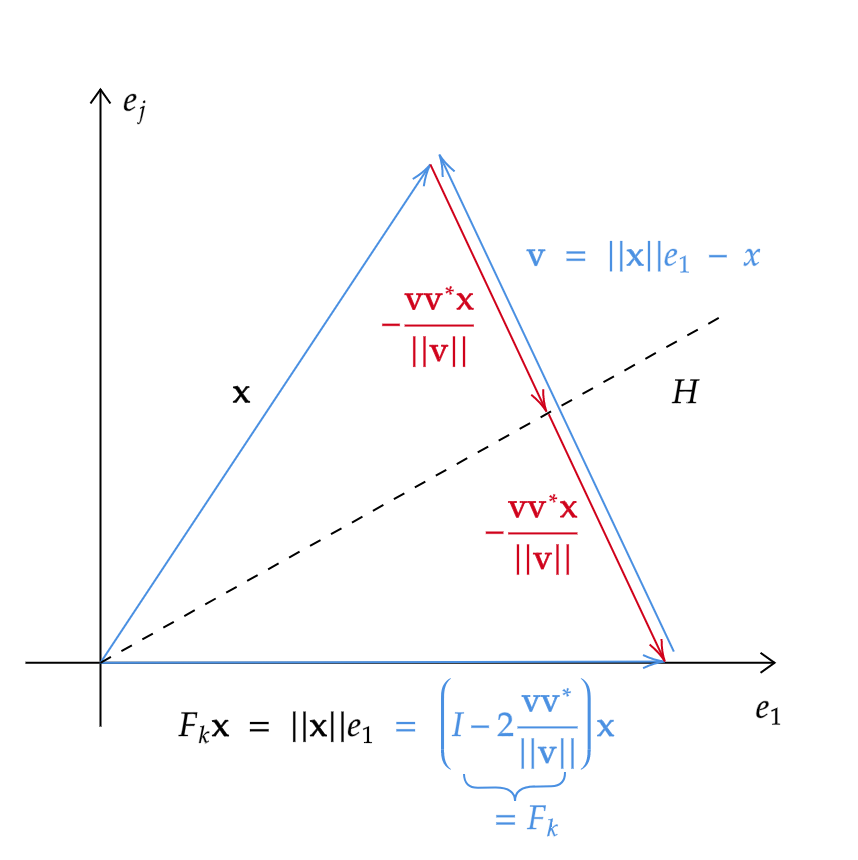
\includegraphics[width=0.7\textwidth]{./imgs/householder-reflector-complete.png}
  \caption{Householder Reflector Explanation}
  \label{fig:householder-reflector-complete}
\end{figure}
\noindent The construction of $\hat{Q}_k$ has been completed with the general structure
\[
  \hat{Q}_k = \begin{pmatrix} I_{k - 1} & 0 \\ 0 & I - 2\frac{vv^{*}}{v^{*}v} \end{pmatrix} 
\]
The expression is the same when taking the negative sign when setting the value of $F_kx$, in the sense that \(x\)  is projected onto the negative axis (for the case in the diagram). You can check if \(\hat{Q}_{k}\) is unitary by yourself. \medskip

\noindent However, the fact above doesn't mean we could randomly choose the $+/-$ sign in  $F_kx = \pm \|x\|e_1$ and \(v = \pm \|x\|e_1 - x\)  for algorithm implementation. \textbf{We need to take the \(F_kx\) away from the original \(x\) as far as possible.} The choice of v should be
\[
  v = sign(x_1)\|x\|e_1 + x
\]   
\textbf{This doesn't seem to make any sense at all.} At least this is what I was thinking when I first looked at this expression. Let me demonstrate the term "as far as possible" and the choice of \(v\)  a little bit:
\begin{itemize}
  \item Note that in the example above, we are projecting vector $x$ to \textbf{the direction that the $+/-$ sign  $x_1$ belongs to.}
  \item That is to say, assuming the first element in $x$ is positive, we are projecting x to the positive direction along the $e_1$ axis, which is the same as we do in \autoref{fig:householder-reflector-initial}, and vice versa.
  \item However this is not a good practice. Let us consider the case that the original vector $x$ is close to the $e_1$ axis and $ \|x\|$ is large. 
    \begin{figure}[H]
      \centering
      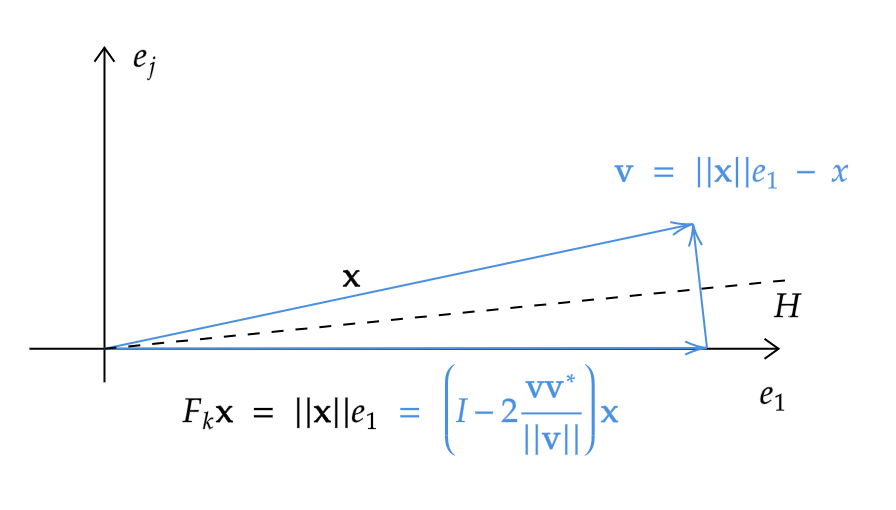
\includegraphics[width=0.7\textwidth]{./imgs/householder-reflector-extreme-case.png}
      \caption{Extreme case when $x$ is close to the $e_1$ axis}
      \label{fig:householder-reflector-extreme-case}
    \end{figure}
  \item In our previous approach we try to obtain $v$ via the difference between $x$ and $sign(x_1)\|x\|e_1$, so in this case, \textbf{the entries in $v$ will be generally small, especially the first entry.}
  \item So here we encounter the case that "two big things give out a small thing" - which is not preferable in computation. The reason is that the small entries in $v$ will trigger the rounding error by inexact arithmetic running on the computer, and \textbf{when $v$ is multiplied by a "big" $x$ the error in the result will be even larger.}
  \item Indeed this situation will lead to the instability of the algorithm, so we cannot project \(x\) to the direction that the $+/-$ sign  $x_1$ belongs to. Therefore, we \textbf{choose the vector further away from the original \(x\),} which is \(-sign(x_1)\|x\|e_1\).
  \begin{figure}[H]
    \centering
    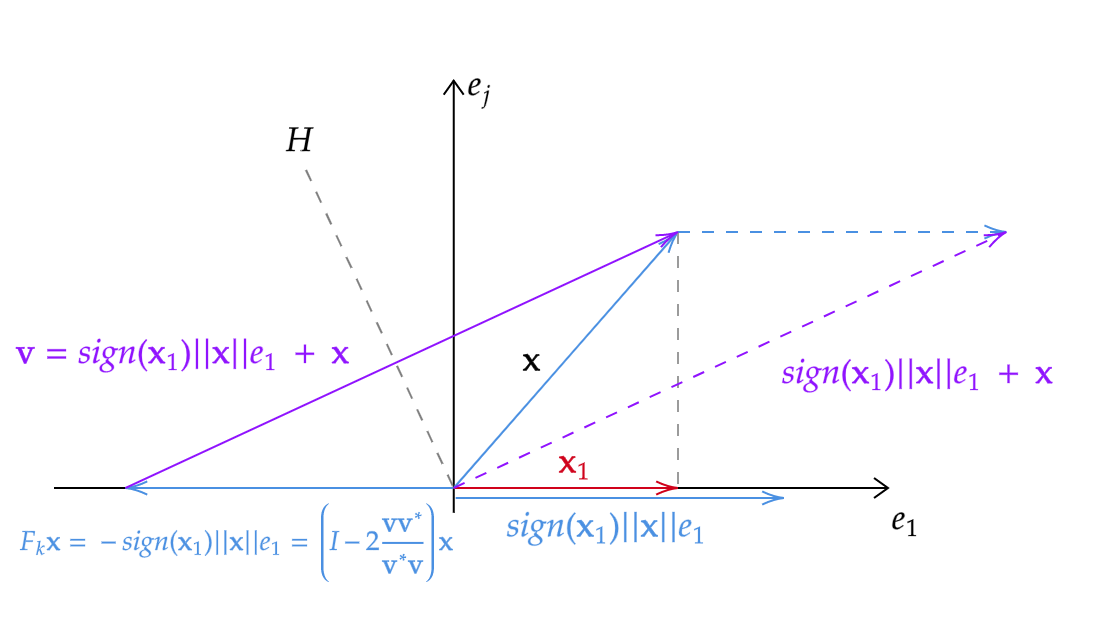
\includegraphics[width=0.7\textwidth]{./imgs/householder-reflector-proper.png}
    \caption{Proper Householder Reflector Construction}
    \label{fig:householder-reflector-proper}
  \end{figure}
  \item Therefore, we update the expression of $v$ due to our different choice of projected vector $F_kx$ by  $v = sign(x_1)\|x\|e_1 + x$, and the expression of \(F_k\) we derived earlier still holds. \autoref{fig:householder-reflector-proper} should be self-intuitive to demonstrate the derivation of $v$ properly.
  \item Note that we have \(sign(0) = 1\)  by convention, and for any \(a \in \mathbb{C}\), \(sign(a) = \frac{a}{|a|}\). You are not encouraged to use \texttt{np.sign()} for implementation, since \texttt{np.sign(0)}\(=0\) and \texttt{np.sign(a)} \(=\frac{a}{Re(a)} \forall a \in \mathbb{C}\).     
\end{itemize}
Now we should have all the background knowledge for householder triangulation. We will not rush to implement QR factorisation with the householder but look at a simple example to "in-place-ly" convert \textbf{the first \(k\)  columns} of a general matrix \(A\) to upper-triangular.

\begin{algorithm}[H]
  \caption{Householder Triangulation}
  \label{alg:householder}
  \begin{algorithmic}[1]
  \Procedure{Householder}{$A$, $k$=None}
  \State $m, n = A$.shape
  \If{$k$ is None}
    \State $k = n$  \Comment{By default we make the whole $A$ upper triangular}
  \EndIf
     \For{ \(i = 1\) to \(k\)}
         \State $x = A$\texttt{[i:, i]}
         \State $e_1 = $ zeros$(len(v))$
         \State $e_1$\texttt{[0]} $= 1$ \Comment{Construct $e_1$ for each iteration}
         \State $v = sign(x_1)\|x\|e_1 + x$
         \State $A$\texttt{[i:, i:]}$ = (I - 2\frac{vv^{*}}{v^{*}v})A\texttt{[i:, i:]}$
     \EndFor
    \State \Return \(A\) 
  \EndProcedure
  \end{algorithmic}
\end{algorithm}
\noindent Note that in \autoref{alg:householder} we are computing the value of $\hat{Q}_{k}\hat{Q}_{k-1}\ldots \hat{Q}_2 \hat{Q}_1A$, but we didn't actually multiply the whole $\hat{Q}_i$ to $A$ in the algorithm as proposed earlier. We multiply the constructed $F = I - 2\frac{vv^{*}}{v^{*}v}$ to the sub-matrix $A$\texttt{[i:, i:]} instead. \medskip

\noindent Obviously, these two operations do the same job and using $F$ is more memory-efficient since we don't need extra spaces for storing 0 and 1 in the identity matrix and zero parts of $\hat{Q}_{i}$.
\subsection*{Exercise 2.8: Implement the Householder Triangulation Algorithm}
\addcontentsline{toc}{subsection}{Exercise 2.8: Implement the Householder Triangulation Algorithm}
\subsubsection*{Problem Description}%
You are now asked to implement the householder triangulation algorithm in \href{https://comp-lin-alg.github.io/cla_utils.html#cla_utils.exercises3.householder}{\texttt{exercises3.householder()}}, to make the first \(k\)  columns in matrix \(A\)  upper-triangular and return the resulted matrix. You should be able to implement it with reference of \autoref{alg:householder}. \medskip

\noindent \textbf{Remember to check your implementation passes the provided test cases.} \medskip

\noindent We can use the algorithm above to perform QR factorization.
\begin{algorithm}[H]
  \caption{QR Factorisation with Householder Triangulation}
  \label{alg:householder-qr}
  \begin{algorithmic}[1]
  \Procedure{Householder\_qr}{$A$}
  \State $m, n = A$.shape
  \State \(A_{aug} = (A|I_m)\)  
  \State \(A_{aug}^{'} = \) HOUSEHOLDER\((A_{aug}, n)\)  
  \State \(R, Q^{*} = A_{aug}^{'}\texttt{[:, :n]}, A_{aug}^{'}\texttt{[:, n:]}\)  
  \State \(Q = (Q^{*})^{*}\)  
    \State \Return \(Q, R\) 
  \EndProcedure
  \end{algorithmic}
\end{algorithm}
\noindent The reason \autoref{alg:householder-qr} works is based on the fact that, function \texttt{HOUSEHOLDER(A, k)} returns the value of \(Q^{*}A\), where \(Q^{*} = \hat{Q}_{k}\hat{Q}_{k - 1}\dots \hat{Q}_{2}\hat{Q}_{1} \in \mathbb{C}^{m\times m}\)  . Furthermore, we could see given that \(D = (B | C)\) is an augmented matrix, where \(B \in \mathbb{C}^{m\times n}, C \in \mathbb{C}^{m\times m}\). Then the result returned by \texttt{HOUSEHOLDER(D, n)} is essentially \((Q^{*}B | Q^{*}C)\), and \(Q^{*}B\) is indeed upper triangular.  \medskip

\noindent Therefore, if we set \(B = A, C = I_{m}\) the case is exactly matched with \autoref{alg:householder-qr}, and the result after householder triangulation would be \((Q^{*}A|Q^{*})\). Since \(R = Q^{*}A\) we have mentioned earlier, now we should have \(R\)  and \(Q^{*}\) in our resulted augmented matrix, and we could easily find values \(Q, R\).

\subsection*{Exercise 2.11: QR Factorisation with Householder Triangulation}
\addcontentsline{toc}{subsection}{Exercise 2.11: QR Factorisation with Householder}
\subsubsection*{Problem Description}%
You are now asked to implement the householder triangulation algorithm in \href{https://comp-lin-alg.github.io/cla_utils.html#cla_utils.exercises3.householder_qr}{\texttt{exercises3.householder\_qr()}}, to return matrices \(Q, R\)  such that \(A = QR\) with householder triangulation. You should be able to implement it with reference of \autoref{alg:householder-qr}. \medskip

\noindent \textbf{Remember to check your implementation passes the provided test cases.} 

\noindent From the exercise above we can learn by analogy to apply householder triangulation to other problems. Say we want to solve a linear system where \(Ax = b, A \in  \mathbb{C}^{m \times  m}, b \in \mathbb{C}^{m}\). \textbf{Note here the RHS is not limited to be a vector,} it could also be a matrix \(\in \mathbb{C}^{m \times k}\). The logic for solving such systems will be the same, except in the matrix case our $x$ is a matrix as well. \medskip

\noindent In this case we could take the same technique in \autoref{alg:householder-qr} to apply \texttt{householder()} on the augmented matrix $(A | b)$ to get the resulted matrix $(R := Q^{*}A | Q^{*}b)$. Now we have re-formulated the equation to $Rx = Q^{*}b = y$, where $R$ is an upper triangular matrix and how to solve such equations computationally is the challenge we need to face now. \medskip

\noindent Now we should have \(R \in \mathbb{C}^{m \times m}\) and \(y \in \mathbb{C}^{m \times  m}\), after expanding the equation $Rx = y$ we will find
\[
\left\{
  \begin{array}{rcl}
    r_{11}x_1 + r_{12}x_2 + \ldots + r_{1(m - 1)}x_{m - 1} + r_{1m}x_{m} & = & y_1 \\
    0x_1 + r_{22}x_2 + \ldots + r_{2(m - 1)}x_{m - 1} + r_{2m}x_m & = & y_2 \\
     & \vdots &  \\
    0x_1 + 0x_2 + \ldots + r_{(m - 1)(m - 1)}x_{m - 1} + r_{(m - 1)m}x_{m} & = & y_{m - 1} \\
    0x_1 + 0x_2 + \ldots + 0x_{m - 1} + r_{mm}x_{m} & = & y_{m}
  \end{array}
\right.
\]
And we could solve this system of linear equations "backwards", starting from the last equation $r_{mm}x_{m} = y_{m}$. Clearly the solution is $x_{m} = \frac{y_{m}}{r_{mm}}$. We now could substitute the value of $x_{m}$ into the previous equation $r_{(m - 1)(m - 1)}x_{m - 1} + r_{(m - 1)m}x_{m} = y_{m - 1}$, to get the value of $x_{m - 1}$. We could use this strategy and go above and above to get all values of $x_{i}, x_{i - 1}, \ldots, x_{2}, x_1$. \medskip

\noindent We call this procedure \textbf{back substitution}, and in general given that we have $x_{i + 1}, x_{i + 2}, \ldots, x_{m - 1}, x_{m}$, we could obtain $x_{i}$ via
\[
x_{i} = \frac{y_{i} - \sum_{k=i + 1}^{m} r_{ik}x_{k}}{r_{ii}} = \frac{y_{i} - (r_{i}^{(i + 1)})^{\top} x^{(i + 1)}}{r_{ii}}
\] 
where $r_{i}^{(i + 1)} = \begin{pmatrix} r_{i(i + 1)} & r_{i(i + 2)} & \ldots & r_{i(m - 1)} & r_{im} \end{pmatrix} ^{\top}$ 

\noindent and $x^{(i + 1)} = \begin{pmatrix} x_{i + 1} & x_{i + 2} & \ldots & x_{m - 1} && x_{m} \end{pmatrix}^{\top} $. \medskip

\noindent And the back substitution algorithm is implemented in this way:

\begin{algorithm}[H]
  \caption{Back Substitution Algorithm for solving \(Rx = y\), special case}
  \label{alg:back-sub-special}
  \begin{algorithmic}[1]
  \Procedure{solve\_U}{$R, y$}
  \State $m, n = R$.shape
  \State Initialise \(x\) as a length-\(m\) vector  
  \For {\(i = m\) to \(1\)}
    \State \(x_{i} = \frac{y_i - (r_i^{(i + 1)})^{\top}x^{(i + 1)}}{r_{ii}}\)  
  \EndFor
    \State \Return \(x\) 
  \EndProcedure
  \end{algorithmic}
\end{algorithm}
\subsection*{Exercise 2.9-10: Solving Systems of Linear Equations}
\addcontentsline{toc}{subsection}{Exercise 2.9-10: Solving Systems of Linear Equations}
\subsubsection*{Problem Description}%
You are now asked to implement the algorithms to solve linear systems
\begin{itemize}
  \item \(Rx = y\)  where \(R \in \mathbb{C}^{m \times m}\), \(R\)  upper triangular, \(y \in \mathbb{C}^{m}\)     
  \item \(AX = B\), where \(A \in \mathbb{C}^{m \times m}, b \in \mathbb{C}^{m \times k}\), and the column vectors \(x_i\) in \(X\) should satisfy \(A x_i = b_i\).
\end{itemize}
using householder triangulation for \href{https://comp-lin-alg.github.io/cla_utils.html#cla_utils.exercises3.solve_U}{\texttt{exercises3.solve\_U()}} and 

\noindent \href{https://comp-lin-alg.github.io/cla_utils.html#cla_utils.exercises3.householder_solve}{\texttt{exercises3.householder\_solve()}}. You should be able to implement it with reference of the knowledge on the previous page and \autoref{alg:back-sub-special}. \medskip

\noindent \textbf{Remember to check your implementation passes the provided test cases.} \medskip

\noindent After introducing the examples above, here is another application of QR factorisation called \textbf{the least square problem.} The problem states that given \(Ax = b, A \in \mathbb{C}^{m \times n}, b \in \mathbb{C}^{n}\) and generally \(m \geq n\). We want to find vector \(x\) which minimises the error function \(\|Ax - b\|^2 = (Ax - b)^{*}(Ax - b)\). \medskip

\noindent That is to say, we are dealing with an over-determined linear system such that we cannot directly find the solution by solving \(Ax = b\). \medskip

\noindent Essentially the minimiser $\overline{x}$ is found by solving the equation $\hat{R}x = \hat{Q}b$ where \(\hat{Q}, \hat{R}\) are coming from the \textbf{reduced QR factorisation} of \(A\). \medskip

\noindent We can still apply the technique to reduce the original equation to an upper-triangular linear system $Rx = y$, where $R \in \mathbb{C}^{m\times n}, x \in \mathbb{C}^{n}$ and $y \in \mathbb{C}^{m}$. The strategy we want to use here is to reduce the matrix $R$ to a square matrix by truncating rows in matrix \(R\)  and the elements in \(y\)  to make \(y\)   length-\(n\) long. You might find using slices in python is helpful for your implementations, i.e. set \(\hat{R} = R\)\texttt{[:n, :n]} and \(\hat{y} = y\)\texttt{[:n]}.


\subsection*{Exercise 2.12: Solving the Least Square Problem}
\addcontentsline{toc}{subsection}{Exercise 2.12: Solving the Least Square Problem}
\subsubsection*{Problem Description}%
You are now asked to implement the algorithm to solve the least square problem $\min \|Ax - b\|^2$
using householder triangulation for 

\noindent \href{https://comp-lin-alg.github.io/cla_utils.html#cla_utils.exercises3.householder_ls}{\texttt{exercises3.householder\_ls()}}. You should be able to implement it with reference of the knowledge above, \texttt{householder\_solve()} and \autoref{alg:back-sub-special}. \medskip

\noindent \textbf{Remember to check your implementation passes the provided test cases.} \bigskip

\noindent Thank you for finishing the reading and reaching this part. One-third of your journey in the course has been completed. Congratulations! \medskip

\noindent Next week you will be facing the first assessed coursework, make sure you manage your time wisely and do ask me questions immediately if you are stuck with one question longer than 1 hour. I will also try my best to provide some sample questions for you to get familiar with the style of coursework questions. \medskip

\noindent Also, \textbf{do make sure you have committed your coding exercises to GitHub} before the coursework deadline, otherwise you will \textbf{lose 35\% of your mark in the first coursework}. Good luck!

\begin{center}
  \textit{\large End of Week 3}\\
  \medskip
  \textit{\large End of Chapter 2}
\end{center}
